\section{Computing a rectification function}\label{rect}

%% This paper considers single-fix rectification of integer arithmetic circuits. We define single-fix rectification as follows:

%% \begin{Definition}
%% Single  fix-rectification  at  target  net $x_i$ means  that  there  exists  a  polynomial  function $U(X_{PI})$ which,  when implemented  at  net $x_i$,  ensures  that circuit $C$ correctly implements the specification $f$.
%% \end{Definition}

%% In \cite{utkarsh:fmcad18}, a rectification check theorem (Theorem V.1) was presented to confirm if a net $x_i$ admits single-fix rectification. This rectification check was presented for finite field arithmetic circuits. However, this theorem can be extended to the model used for integer arithmetic circuits. In this paper, we assume that the theorem is applied to a net $x_i$, where single-fix rectification is found to be possible. Given such a net $x_i$, we compute a rectification polynomial which can be implemented at that net to rectify the circuit. 

Assume that post-verification debugging has been performed and a net
$x_i$ in the circuit $C$ has been identified that admits single-fix
rectification. Therefore, our objective is to now compute a function
$x_i = U(X_{PI})$ such that $U: \{0,1\}^{|X_{PI}|}\rightarrow
\{0,1\}$. We will first show how to compute $U$ as a polynomial
function, and then how to synthesize it as a circuit. Polynomially, we
will represent the hitherto unknown component $U$ as $f_i = x_i -
U(X_{PI})$, where $x_i$ is the leading term of the corresponding
polynomial. 


% \subsection{Problem Statement}

% \begin{itemize}
%     \item Given $R = \Q[x_1,\dots,x_n]$.
%     \item Given a word-level specification polynomial $f$.
%     \item Given a buggy $k$-bit integer multiplier circuit $C$. The bit-level primary inputs are $\{a_0,\dots,a_{k-1}\}$ and $\{b_0,\dots,b_{k-1}\}$. The bit-level primary outputs are $\{z_0,\dots,z_{2k-1}\}$.
%     \item Analyze the topology of the circuit and derive RTTO.
%     \item Given a system of polynomial equations modeling the gates in the circuit $C$, $F=\{f_1,\dots,f_s\}\subset R = \Q[x_1,\dots,x_n]$ and the set $F_0=\{x_1^2-x_1,\dots,x_n^2-x_n\}$.
%     \item Given a net $x_i$ which admits single-fix rectification.
% \end{itemize}

% Our goal is to find a polynomial function $x_i = U(X_{PI})$ that maps $\{0,1\}^{|X_{PI}|} \rightarrow \{0,1\}$, such that $f \in \langle f_1,\dots,f_i:x_i-U(X_{PI}),\dots,f_s,x_1^2-x_1,\dots,x_n^2-x_n \rangle$. This polynomial function rectifies the circuit.

%\subsection{Procedure to compute rectification function}

Let $R = \Q[x_1,\dots,x_n]$ and let $F =
\{f_1,\dots,f_i:x_i-U(X_{PI}),\dots,f_s\}$ the system of polynomials
modeling the correct circuit and $U(X_{PI})$ is the unknown
rectification polynomial to be computed. The polynomials are ordered
according to RTTO, s.t. $lt(f_1) > lt(f_2) > \dots > lt(f_i):x_i
> lt(f_{i+1}) > \dots > lt(f_s)$. The desired rectification function
$U(X_{PI})$ computed must satisfy the condition $f \in \langle
f_1,\dots,f_i:x_i-U(X_{PI}),\dots,f_s,x_l^2-x_l \rangle$, where $x_l
\in X_{PI}$. This polynomial function $U(X_{PI})$ can be computed
using the combination of extended \Grobner Basis and ideal membership
testing. As the polynomial $f_i = x_i-U$ corrects the circuit, we can write:
\vspace{-1mm}
\begin{equation}
\label{eq:eqn1}
%\begin{split}
   f \in \langle  f_1,\dots,f_{i-1},\boldsymbol{f_i: x_i - U},f_{i+1},\dots,f_s,  x_l^2-x_l \rangle 
%\end{split}
\end{equation}

The ideal membership relation of $f$ can be written as:
\vspace{-0.5mm}
\begin{equation}
    \label{eq:eqn2}
\begin{split}
f = & h_1f_1 + h_2f_2 + \dots+\boldsymbol{h_if_i}+\dots+h_sf_s \\
& + \sum_{x_l \in X_{PI}} H_l
\cdot(x_l^2-x_l)    
\end{split}
\end{equation}

where $\{h_1,\dots,h_s,H_l\} \subset R$ are arbitrary polynomials. Substituting $f_i = x_i - U$:
\vspace{-1mm}
\begin{equation}
\begin{split}
    f = & h_1f_1 + h_2f_2 + \dots+\boldsymbol{h_i(x_i-U)}+\dots+h_sf_s \\
    & + \sum_{x_l \in X_{PI}} H_l \cdot(x_l^2-x_l)
\end{split}
\end{equation} 
\vspace{-0.25in}

\begin{equation}
\begin{split}
 f = & h_1f_1 + h_2f_2 + \dots+\boldsymbol{h_ix_i-h_iU}+\dots+h_sf_s \\
 & + \sum_{x_l \in X_{PI}} H_l \cdot(x_l^2-x_l)   
\end{split}
\label{eq:eqn3}
\end{equation}

\vspace{-0.15in}

\begin{equation}
\label{eq:eqn4}
\begin{split}
   & f - h_1f_1 - h_2f_2 - \dots-h_ix_i \\
   & = -h_iU+\dots+h_sf_s + \sum_{x_l \in X_{PI}} H_l \cdot(x_l^2-x_l) 
\end{split}
\end{equation}

%\vspace{-0.1in}

Notice that on the L.H.S. of Eqn. (\ref{eq:eqn4}), the polynomials
$f, f_1,\dots,f_{i-1}$ and the monomial $x_i$ are known polynomial expressions. Therefore, $f$ can be divided by $f_1,\dots,f_{i-1}$ and $x_i$ to obtain the respective quotients of the division
$h_1,\dots,h_i$ and remainder $r$. The polynomial $f$ can be written as 
\begin{equation}
f = h_1f_1 + h_2f_2 + \dots + h_ix_i + r
\end{equation}
The remainder $r$ can be computed as:
\begin{equation}
r = f - h_1f_1 - h_2f_2 - \dots - h_ix_i
\label{eq:eqnr}
\end{equation}

After $h_i$ is computed (as quotient of division by $x_i$),
the R.H.S. of Eqn. (\ref{eq:eqn4}) consists of $h_i,f_{i+1},\dots,f_s$ and polynomials $x_l^2-x_l$ as known expressions. This
implies:
\vspace{-1mm}
\begin{equation}
f - h_1f_1 - \dots-h_ix_i \in \langle -h_i,f_{i+1},\dots,f_s,  x_l^2-x_l\rangle
\end{equation}
\vspace{-4mm}
\begin{equation}
r \in \langle -h_i,f_{i+1},\dots,f_s,  x_l^2-x_l\rangle
\label{eq:eqn5}
\end{equation}

Note that RTTO renders the polynomial $f_{i+1},\dots,f_s$ a \Grobner
Basis. However, $\{-h_i,f_{i+1},\dots,f_s\}$ is not. We compute its a
\Grobner Basis $G = \{g_1,\dots, g_t\}$. We apply the extended
\Grobner Basis theory explained in Eqn. (\ref{eqn:imt_orig}) to $G$ to
find the ideal membership relation of $r$. 

\vspace{-0.15in}

\begin{equation}
    r = -h_i'h_i+h_{i+1}'f_{i+1}+\dots+h_s'f_s+ \sum_{x_l \in X_{PI}} H_l' (x_l^2-x_l)
    \label{eq:eqn6}
\end{equation}

Then $h_i'$ is a polynomial that satisfies the ideal membership
relation in Eqn. (\ref{eq:eqn1}). According to \cite{utkarsh:fmcad18},
the polynomial $h_i' = U$  rectifies the circuit such that the circuit
matches the specification.   

However, in our model, $h_i'$ is computed over the field of
rational numbers $\Q$. This polynomial may have fractional
coefficients and it may also evaluate to any non-Boolean value in $\Q$
for some primary input vectors. We use the example of a 3-bit
multiplier shown in Fig. \ref{fig:3appmult} to explain this in more
detail.  

\begin{figure}[H]
    \centering
    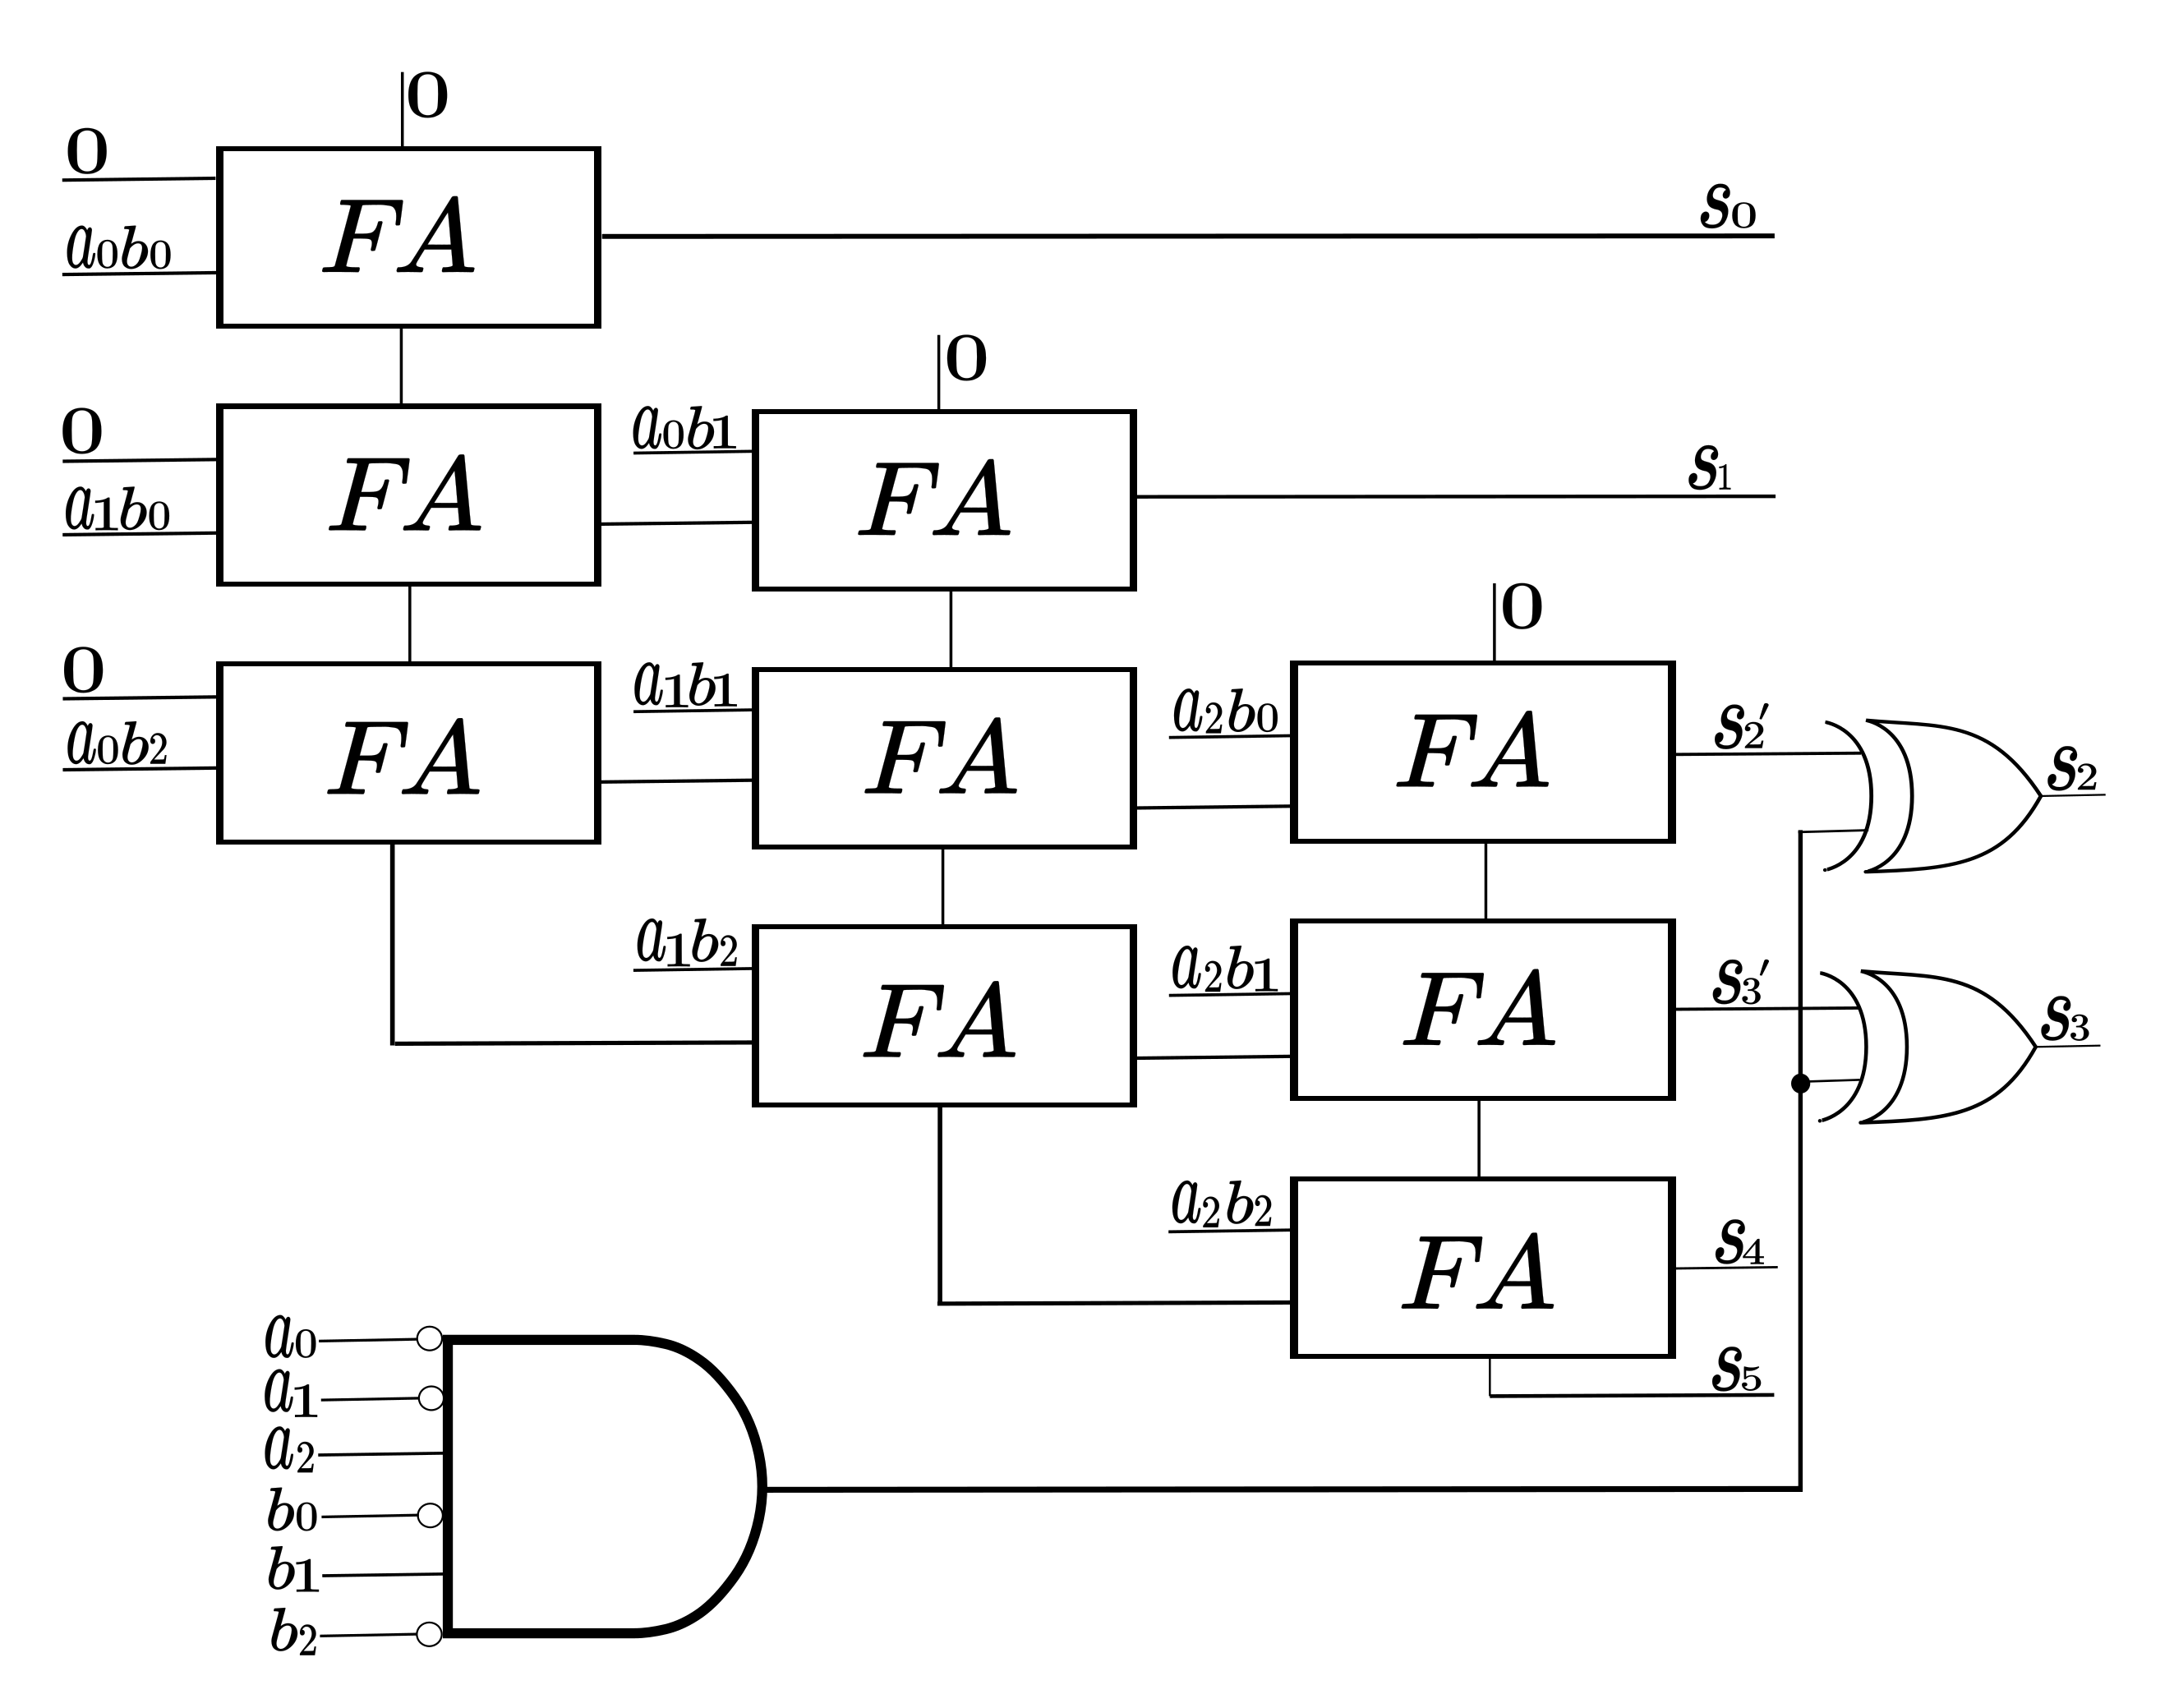
\includegraphics[scale = 0.06]{3appmult.png}
    \caption{3-bit multiplier with additional circuit to introduce a bug}
    \label{fig:3appmult}
\end{figure}

\begin{Example}
The Fig. \ref{fig:3appmult} shows a 3-bit array multiplier circuit. A
bug in introduced in the circuit in the form of additional gates as
shown. Gates are added to the circuit to modify the function of the
circuit at two output bits for one input pattern
$(a_0,a_1,a_2,b_0,b_1,b_2)=(0,0,1,0,1,0)$. Single-fix
rectification is feasible at a net $n_{22}$ in the 
circuit. We apply Eqns. (\ref{eq:eqn1}) to (\ref{eq:eqn6}) and compute
the rectification function $h_i'$, as well as $h_i$, as shown in
Eqn. (\ref{eq:eqn4}).  
{\small
\begin{equation}
    \begin{split}
h_i & = 8\cdot a_0\cdot a_1\cdot a_2\cdot b_0
+16\cdot a_0\cdot a_1\cdot a_2\cdot b_1
-12\cdot a_0\cdot a_1 \\
& -8\cdot a_0\cdot a_2\cdot b_0 
 -16\cdot a_0\cdot a_2\cdot b_1 
 +12\cdot a_0-8\cdot a_1\cdot a_2\cdot b_0 \\
& -16\cdot a_1\cdot a_2\cdot b_1 
+12\cdot a_1+8\cdot a_2\cdot b_0
+16\cdot a_2\cdot b_1
-12        
    \end{split}
    \nonumber
\end{equation}

\begin{equation}
    \begin{split}
h_i' = & -\frac{44}{3}\cdot a_0\cdot a_1\cdot a_2\cdot b_0\cdot b_1\cdot b_2+
\frac{4}{3}\cdot a_0\cdot a_1\cdot a_2\cdot b_0\cdot b_1 \\
& +8\cdot a_0\cdot a_1\cdot a_2\cdot b_0\cdot b_2
+\frac{8}{3}\cdot a_0\cdot a_1\cdot a_2\cdot b_1\cdot b_2 \\
& +\frac{4}{3} \cdot a_0\cdot a_1\cdot b_0\cdot b_1\cdot b_2
-\frac{2}{3}\cdot a_0\cdot a_1\cdot b_0\cdot b_1 \\
&+\frac{4}{3}\cdot a_0\cdot a_1\cdot b_1\cdot b_2
+\frac{8}{3}\cdot a_0\cdot a_2\cdot b_0\cdot b_1\cdot b_2 \\
& -4\cdot a_0\cdot a_2\cdot b_0\cdot b_2 
+\frac{28}{3}\cdot a_1\cdot a_2\cdot b_0\cdot b_1\cdot b_2 \\
& -\frac{14}{3}\cdot a_1\cdot a_2\cdot b_0\cdot b_1
-\frac{8}{3}\cdot a_1\cdot a_2\cdot b_0\cdot b_2 \\
&-\frac{20}{3}\cdot a_1\cdot a_2\cdot b_1\cdot b_2
+\frac{8}{3}\cdot a_1\cdot a_2\cdot b_1 \\
&-\frac{2}{3}\cdot a_1\cdot b_1 
-\frac{4}{3}\cdot a_1\cdot b_2
+1        
\end{split}
\nonumber
\end{equation}
}

We evaluate the polynomial $h_i$ and $h_i'$ for all primary input patterns. The observations are recorded in the following table. 
\vspace{2mm}
\begin{table}[ht]
    \centering
    \begin{tabular}{|c|c|c|} \hline
      $a_0,a_1,a_2,b_0,b_1,b_2$ & $h_i$ & $h_i'$ \\ \hline
       0,0,0,0,0,0 & -12 & 1\\ \hline
       0,0,0,0,0,1 & -12 & 1\\ \hline
       0,0,0,0,1,0 & -12 & 1\\ \hline
       0,1,0,0,0,1 & 0 & $-\frac{1}{3}$\\ \hline
       0,1,0,0,1,0 & 0 & $\frac{1}{3}$\\ \hline
       0,1,0,0,1,1 & 0 & -1 \\ \hline
    \end{tabular}
    \caption{Evaluating $h_i$ and $h_i'$}
    \label{tab:quosol}
\end{table}

In order to conserve space, Table \ref{tab:quosol} shows the data for
only some input patterns.
%We make some observations based on the contents of this table.
The rectification polynomial $h_i'$ has
fractional coefficients. At points where $h_i = 0$, we see that $h_i'$
can evaluate to any value in $\Q$. We found 48 such points where $h_i$
evaluates to 0. At points where $h_i \neq 0$, we always observe that $h_i'$
evaluates to a value in $\{0,1\}$. 
\end{Example}

%Consider the polynomial $h_i$ which is computed as a quotient of
%division by $x_i$ in Eqn. (\ref{eq:eqn4}). We can see that the
%rectification polynomial $h_i'$ depends on the polynomial $h_i$. This
%is also confirmed by the data shown in Table \ref{tab:quosol}.
In order to understand the conditions under which the rectification
polynomial $h_i'$ computes to only Boolean values, we investigate at the
variety of $h_i$. We make the following claims:

%% Let us assume there exists a polynomial $U$, which
%% can be implemented at net $x_i$ to rectify the circuit. This
%% polynomial is a Boolean polynomial, which performs the mapping
%% $\{0,1\}^{|X_j|} \rightarrow \{0,1\}$, where $X_j$ is the set of
%% variable that are less than $x_i$ in RTTO. This polynomial can be
%% reduced to the primary input variables, $U(X_{PI})$. The existence of
%% such a polynomial can be confirmed by performing the rectification
%% check at $x_i$, shown in \cite{utkarsh:fmcad18}.  
%% % \vspace{2mm}

%% Based on these assumptions, 

\begin{Fact}
The polynomials $h_i$ and $h_i'$ are computed in terms of variables in
the set $X_j$, where $X_j < x_i$ in RTTO.  
\end{Fact}

We use \Grobner basis division to compute $h_i$. This division is
shown in Eqn. (\ref{eq:eqn4}). The order of division under RTTO
ensures that $h_i$ is a polynomial in those variables which are less
than $x_i$ in the term order. Similarly, the extended \Grobner basis
algorithm used to compute $h_i'$ in Eqn. (\ref{eq:eqn6}),
ensures that $h_i'$ is a polynomial in those variables which are less
than $x_i$ in the term order. 


%% \begin{Fact}
%% The polynomial $h_i'$ is computed in terms of variables in the set $X_j$, where $X_j < x_i$ in RTTO. 
%% \end{Fact}

\begin{Fact}
{\small 
  \begin{equation}
    h_i(U-h_i') = \sum_{j = i+1}^{s} (h_j-h_j')f_j+\sum_{x_l\in X_{PI}}(H_l-H_l')(x_l^2-x_l)
    \label{eq:eqn7}
\end{equation}
}
\end{Fact}

We get Eqn. (\ref{eq:eqn7}) by combining Eqns. (\ref{eq:eqn4}), (\ref{eq:eqnr}) and (\ref{eq:eqn6}).

\begin{Fact}
  Let $p \in \{0,1\}^{|X_{PI}|}$ be an assignment to the primary
  inputs of $C$. Let $p'$ be the assignment to the all the nets in $C$
  under the application of $p$ to $X_{PI}$; denote $p'|_{X_{PI}} = p$
  as the projection of $p'$ to primary inputs. Then, we have $\forall
  p \in \{0,1\}^{|X_{PI}|},\ \exists p'$, such that $p'|_{X_{PI}} = p$
  and $f_{i+1}(p') = \dots = f_s(p') = 0$. 
\end{Fact}

Clearly, for all primary input assignments, there exists an assignment
to the nets that satisfies all the gates of the circuit. By using the
three facts stated above, we state and prove the following results:

% \begin{Theorem}
% Let point $p \in \{0,1\}^{|X_{PI}|}$ be a point.\\
% (i) If $h_i(p) = 0$, i.e., $p \in V(\langle h_i \rangle + J_0)$, then $h_i'(p)$ evaluates to a value in $\Q$.\\
% (ii) If $h_i(p) \neq 0$, i.e., $p \notin V(\langle h_i \rangle + J_0)$, then $h_i'(p) \in \{0,1\}$.
% \label{thm:quo2}
% \end{Theorem}

\begin{Theorem}
Let there exist a polynomial $U$ that maps from $\{0,1\}^{|X_j|}
\rightarrow \{0,1\}$. Let $p'$ be a point in the affine space such
that $p'|_{X_{PI}} = p$ and $f_{i+1}(p') = \dots = f_s(p') = 0$. If
$h_i(p') \neq 0$, then $h_i'(p) = U(p')$. 
\label{thm:quo}
\end{Theorem}

\textbf{Proof:}
Consider Eqn. (\ref{eq:eqn7}) and point $p'$ such that
$p'|_{X_{PI}}$, and $f_{i+1}(p') = \dots = f_s(p') = 0$. We know that
$x_l^2 = x_l$ at any point $p \in \{0,1\}^{|X_{PI}|}$. Therefore,
R.H.S. of Eqn. (\ref{eq:eqn7}), when evaluated at $p'$, is 0. Then, we
have $h_i(p')(U(p') - h_i'(p')) = 0$.
In L.H.S. of Eqn. (\ref{eq:eqn7}), when $h_i(p') \neq 0$, $U(p') = h_i'(p')$. 

Since we know (or have assumed) that there exists a (Boolean)
rectification function $U$ for $C$ at $x_i$, we know that $U(p')$
evaluates to a value in $\{0,1\}$. Therefore, according to Theorem
\ref{thm:quo}, $h_i'$ evaluates to a Boolean value at those points
where $h_i \neq 0$.  


\begin{Corollary}
Let point $p$ be such that $p \in \{0,1\}^{|X_{PI}|}$. Let $p'$ be a
point such that $p'|_{X_{PI}} = p$. If $h_i(p') = 0$, the polynomial
$h_i'$ can be modified such that $h_i'(p')$ evaluates to a value in
$\{0,1\}$. 
\end{Corollary}

\textbf{Proof:} Consider Eqn. (\ref{eq:eqn7}). Consider a point $p'$ such that $p'|_{X_{PI}}$ and $f_{i+1}(p') = \dots = f_s(p') = 0$. We know that $x_l^2 = x_l$ at any point $p \in \{0,1\}^{|X_{PI}|}$. Therefore, R.H.S. of Eqn. (\ref{eq:eqn7}) is 0.
\begin{equation}
    h_i(U - h_i') = 0. 
    \label{eq:hinot0}
\end{equation}
In L.H.S. of Eqn. (\ref{eq:hinot0}), $h_i(p') = 0$. Therefore, $U$ can
take any value in $\Q$ at $p'$ to satisfy Eqn. (\ref{eq:hinot0}).
%it does not depend on $h_i'(p')$. 

The above results imply that $U(X_{PI})$ evaluate to Boolean values
wherever $h_i(p') \neq 0$, and $U(X_{PI})$ may evaluate to non-Boolean
values in $\Q$ where $h_i(p')=0$. However, ideal membership
Eqn. (\ref{eq:eqn4}) is always satisfied when $h_i(p')=0$
(irrespective of the value of $h_i'(p')$). Hence, we can modify
the polynomial function $h_i'=U$ at those points $p$ where $h_i(p) =
0$, to evaluate to any  value in $\{0,1\}$, without affecting the
ideal membership relation in Eqn (\ref{eq:eqn4}). These points $p$
where $h_i(p)=0$ form the {\it don't care} set for the rectification
function.  

%% Due to the compact structure of arithmetic circuits, we usually
%% compute polynomial $h_i$ such that $V(\langle h_i \rangle + J_0) =
%% \emptyset$. This implies that the polynomial $h_i$ does not evaluate
%% to 0 at any point in $\{0,1\}^{|X_{PI}|}$. 

Based on the above discussion, the following claim can also be easily
shown, and is stated without proof.
\begin{Corollary}
\label{thm:quo2}
If $\forall p \in \{0,1\}^{|X_{PI}|}$ and $h_i(p') \neq 0\ \forall p'$
such that $p'|_{X_{PI}} = p$, then polynomial $U$ is unique and can be
computed as polynomial $h_i'$ using Eqns. (\ref{eq:eqn1})-(\ref{eq:eqn6}).  
\end{Corollary}

%\textbf{Proof:} By extension of proof for Theorem \ref{thm:quo}, $U(p') = h_i'(p'),\ \forall p'$.


{\it Overall Rectification Approach:} i) Compute $h_i$ and $U=h_i'$ as
shown in  Eqns. (\ref{eq:eqn1})-(\ref{eq:eqn6}). ii) Compute $G =
GB(h_i, F_0)$. If $G = \{1\}$, then it implies that $h_i$ has no
zeros, i.e. $h_i(p')\neq 0, \forall p' \in \{0,1\}^n$. Then $U=h_i'$ is a
Boolean function and it can be uniquely computed with integral
coefficients. $U$ can then be reduced $\pmod{ 2}$, where the products
terms can be implemented as AND gates, and sum terms as XOR
gates. iii) If $G = GB(h_i, F_0) \neq \{1\}$, then $h_i$ evaluates to
0 at some points. Evaluate $h_i$ for all points $p'$, and where
$h_i(p')=0$, set $h_i'(p)=U(p)$ as {\it don't cares}, and generate a
function table, which can be synthesized and attached to net $x_i$. 











%% Corollary \ref{thm:quo2} can be explained using the following example of a 2-bit integer multiplier shown in Fig. \ref{fig:3mult}.

%% \begin{figure}[H]
%%     \centering
%%     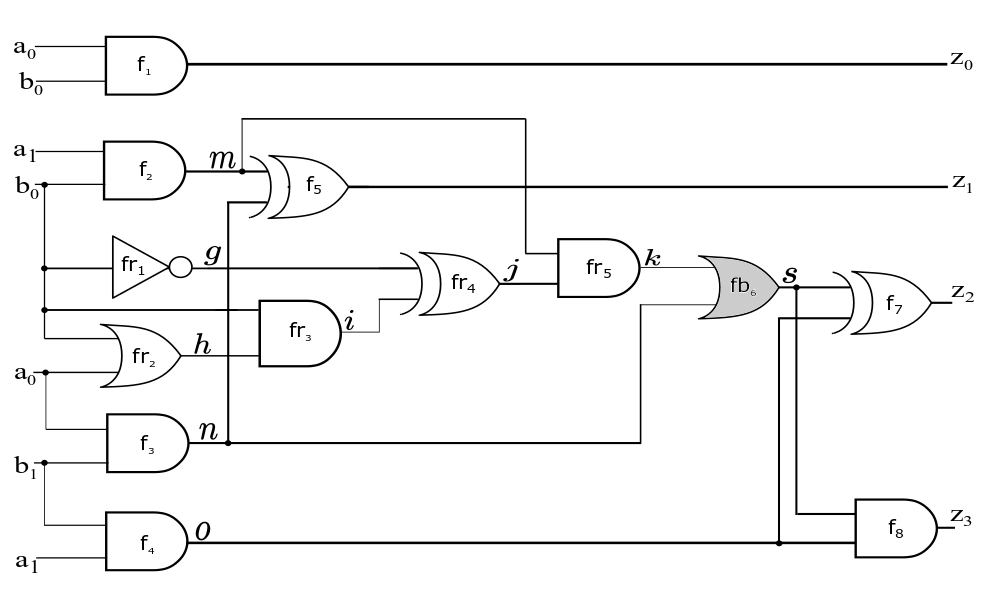
\includegraphics[scale = 0.2]{int_mul_red_b.png}
%%     \caption{2-bit integer multiplier with redundancy with a bug at $s$.}
%%     \label{fig:3mult}
%% \end{figure}
%% \begin{Example}
%% A bug is introduced in the 2-bit integer array multiplier circuit, with added redundancy, shown in Fig. \ref{fig:3mult}. The bug is introduced at a net $s$, which lies in the input cone of the primary outputs $z_2$ and $z_3$. The bug is introduced by replacing the AND gate at $s$ by an OR gate. 



%% \begin{align*}
%% & f_1 = z_0-a_0\cdot b_0 && f_2 = m-a_1\cdot b_0 \\
%% & f_{r1} = g-1+b_0 && f_{r2} = h-a_0-b_0 + a_0\cdot b_0 \\
%% & f_3 = n-a_0\cdot b_1 && f_4 = o-a_1\cdot b_1 \\
%% & f_5 = z_1-m-n+2\cdot m \cdot n && f_{r3} = i-h \cdot b_0 \\
%% & f_{r4} = j-i-g+2 \cdot i \cdot g && f_{r5} = k-j \cdot m \\
%% & \mathbf{f_{b6} = s-k- n+k\cdot n} && f_7 = z_2-s-o+2\cdot s \cdot o \\
%% & f_8 = -z_3+s\cdot o \\
%% \end{align*}

%% The specification for a 2-bit multiplier is:

%% $f = \sum_{i=0}^{2n-1} 2^iz_i-\sum_{i=0}^{n-1} 2^ia_i\cdot \sum_{i=0}^{n-1} 2^ib_i$

%% Verification is done by performing \Grobner Basis reduction, $f \xrightarrow{J+J_0}_+r$.
%% We find $r = -4\cdot a_0\cdot a_1\cdot b_0\cdot b_1+4\cdot a_0\cdot b_1$. Since $r \neq 0$, verification fails and rectification is attempted. Rectification is attempted at net $s$ itself. The procedure to compute a rectification polynomial, shown in Eqns. (\ref{eq:eqn1}) to (\ref{eq:eqn6}), is applied. We compute the following two polynomials. 

%% $$h_i =  4$$

%% \begin{equation}
%% \label{sol}
%% U = a_0\cdot a_1\cdot b_0\cdot b_1
%% \nonumber
%% \end{equation}

%% The polynomial $h_i'$ is the rectification polynomial we computed. The polynomial $h_i = 4$ indicates that it never evaluates to $0$ for any value in $\{0,1\}^{|X_{PI}|}$. Therefore, following Corollary \ref{thm:quo2}, $h_i'$ evaluates to a value in $\{0,1\}$. This is confirmed by evaluating this polynomial for all points in $\{0,1\}^{|X_{PI}|}$. 
%% \label{ex:3bit}
%% \end{Example}

%% The polynomial obtained from our procedure can be synthesized by first reducing it to primary input variables through \Grobner Basis reduction. We compute $U(X_{PI}) \pmod{J+J_0}$. Since this polynomial is a Boolean polynomial, we can find $U(X_{PI}) \pmod{2}$. By interpreting `$+\pmod{2}$' as XOR operation and `$* \pmod{2}$' as AND operation, we can obtain a Reed-Muller form of the rectification function. This AND-XOR expression can be synthesized as a logic circuit by any synthesis tool. 

%% For the rectification polynomial in Example \ref{ex:3bit}, the polynomial was already computed in terms of primary input variables. 

%% The AND-XOR expression for the above rectification function is computed as:

%% $s = a_0\land a_1\land b_0\land b_1$









